\section{Evaluation}
\textbf{Once the screenshot is removed this section may be something we can kill for space.}
The 1-bit adder example network was used to evaluate the framework for correctness. Its truth table was compared to the expected output for all permutations of possible valid inputs. The verified network can be seen in in Figure \ref{1_bit_adder}.
% That means we validated the network on the following inputs following the format (A, B, Carry In) -> (Sum, Carry Out):
% \begin{itemize}
%     \item (0, 0, 0) -> (0, 0)
%     \item (0, 0, 1) -> (1, 0)
%     \item (0, 1, 0) -> (1, 0)
%     \item (0, 1, 1) -> (0, 1)
%     \item (1, 0, 0) -> (1, 0)
%     \item (1, 0, 1) -> (0, 1)
%     \item (1, 1, 0) -> (0, 1)
%     \item (1, 1, 1) -> (1, 1)
% \end{itemize}

The C-MCPN Framework works well for logical operations with a fixed number of inputs and outputs, and the C-MCPN Editor makes it easy to construct and visualize these networks. There were two key insights gained throughout the creation of this framework which are the importance of the edges carrying values and the minimalistic fact structure which improves the performance of the network. This framework is a novel approach to neural network representation within a logical programming paradigm like ASP.

The C-MCPN Editor also shows potential as a powerful educational tool for understanding both neural networks and logic programming. Showing a visualization of the network structure along with a live preview of the code necessary to create it is a great way to help users relate the two ideas. 

\textbf{Editor screenshots should be moved to the preceding section.}
\begin{figure}[h]
    \centering
    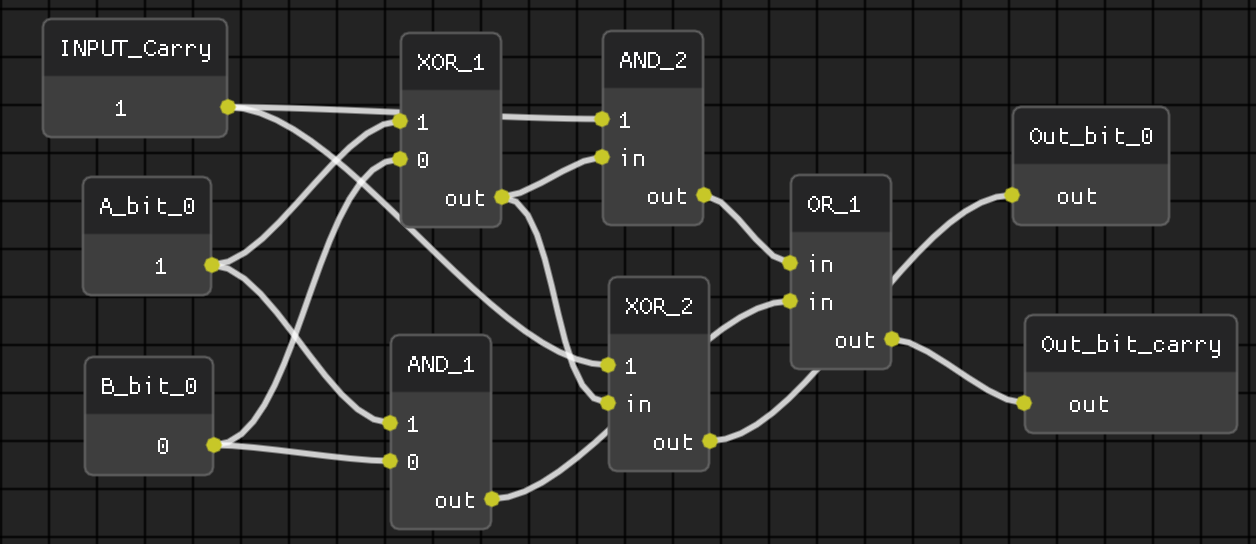
\includegraphics[width=0.8\textwidth]{figures/1-bit adder.png}
    \caption{A screenshot of a 1-bit adder network in the C-MCPN Editor.}
    \label{1_bit_adder}
\end{figure}

\subsection{Limitations}
This work is a proof of concept for the C-MCPN Framework and Editor, and as such there are some limitations to be aware of. The framework has no cycle detection nor has it been tested on recurrent networks. This is likely to cause issues with the value inference program, as it relies on the values being propagated along the edges. The framework has also not been tested on large networks, and it is unknown how scale will affect its performance. It is also worth noting that Clingo does not have native support for floating point numbers, limiting the potential applications of easy to understand networks. 
